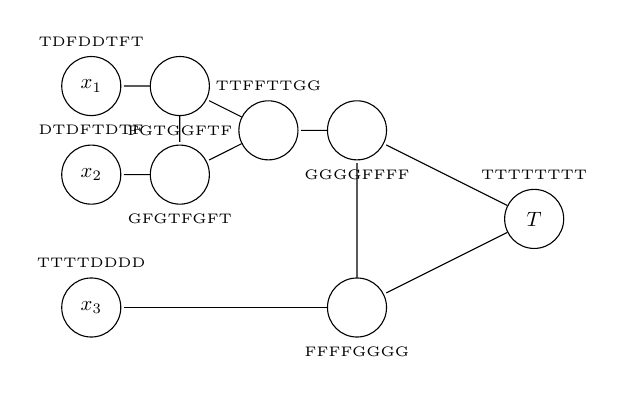
\begin{tikzpicture}[shorten >=1pt,node distance=2cm,auto,scale=1.5,nd/.style={draw=black,circle,scale=\sc,minimum width=0.75 cm,minimum height=1 cm},ndg/.style={nd,fill=gray},yscale=-1,scale=0.75]
\def\sc{0.75}
\node[nd]  (R0) at (0,0)     {$T$};
\node[nd]  (R1) at (-2,1)    {};
\node[nd]  (R2) at (-2,-1)   {};
\node[nd]  (R3) at (-3,-1)   {};
\node[nd]  (R4) at (-4,-1.5) {};
\node[nd]  (R5) at (-4,-0.5) {};
\node[nd]  (R6) at (-5,-1.5) {$x_1$};
\node[nd]  (R7) at (-5,-0.5) {$x_2$};
\node[nd]  (R8) at (-5,1)    {$x_3$};
\foreach \i/\j/\k in {0/1/2,3/4/5} {
  \path (R\i) edge (R\j);
  \path (R\i) edge (R\k);
  \path (R\j) edge (R\k);
}
\foreach \i/\j in {2/3,1/8,4/6,5/7} {
  \path (R\i) edge (R\j);
}
\foreach \i/\a/\b/\t in {0/north/south/TTTTTTTT,1/south/north/FFFFGGGG,2/south/north/GGGGFFFF,3/north/south/TTFFTTGG,4/south/north/FGTGGFTF,5/south/north/GFGTFGFT,6/north/south/TDFDDTFT,7/north/south/DTDFTDTF,8/north/south/TTTTDDDD} {
  \draw (R\i.\a) node[anchor=\b]{\tiny{\t}};
}
\end{tikzpicture}